\documentclass[uplatex,dvipdfmx]{jsarticle}

\usepackage[uplatex,deluxe]{otf} % UTF
\usepackage[noalphabet]{pxchfon} % must be after otf package
\usepackage{stix2} %欧文&数式フォント
\usepackage[fleqn,tbtags]{mathtools} % 数式関連 (w/ amsmath)
\usepackage{hira-stix} % ヒラギノフォント&STIX2 フォント代替定義(Warning回避)
\usepackage{float} % Enables [H] float placement option
\usepackage{listings}
\usepackage{url}
\lstset{
basicstyle={\ttfamily},
identifierstyle={\small},
commentstyle={\smallitshape},
keywordstyle={\small\bfseries},
ndkeywordstyle={\small},
stringstyle={\small\ttfamily}, frame={tb},
breaklines=true, columns=[l]{fullflexible},
numbers=left, xrightmargin=0zw, xleftmargin=3zw,
numberstyle={\scriptsize}, stepnumber=1,
numbersep=1zw, lineskip=-0.5ex
}

\begin{document}

\title{高気温時警告システムの仕様書}
\author{25G1051 近藤巧望}
%\date{2025年7月2日}
\maketitle
\section{本システムの概要}
\indent
近年,気温の上昇に伴い,熱中症のリスクが高まっている.
特に,夏季の高温環境下では,熱中症の発症が増加しており,その予防と対策が重要な課題となっている.
熱中症は,重篤な場合には生命に関わることもあり,一命を取り留めたとしても高次脳機能障害などの後遺症が残ることがあるため非常に危険である.
本人は意外にも自身が熱中症にかかっていることに気づかない事が多く,熱中症への意識を高めることが重要である.
そこで今回,私は高気温時警告システムを提案する.
このシステムは,気温のリアルタイム表示に加え気温が30度を超えた場合にアラームで警告し,熱中症への対策を促すことを目的としている.
これにより,現在の気温が高いことを意識させ,熱中症の予防につなげることができると考えられる.
主に気温検知用の温度センサー,気温のリアルタイム表示用の7セグメントディスプレイ,アラームを鳴らすための圧電ブザー,およびシステム全体を制御するArduino UNO R3で構成される.

\section{本システムの構成}
\subsection{入力・処理・出力の構成}

\begin{table}[H]
  \centering
  \caption{本システムの構成要素}
  \label{table:presentation}
  \begin{tabular}{ccl}
\hline
項目 & 構成 & 役割 \\\hline \hline
1 & 温度センサー[TMP36] & 気温を検知する \\ \hline
2 & 7セグメントディスプレイ(クロック表示) & 気温を表示する \\ \hline
3 & 圧電ブザー & アラームで警告する \\ \hline
4 & Arduino UNO R3 & システム全体を制御する \\ \hline
  \end{tabular}  
\end{table}

\begin{figure}[H]
\centering
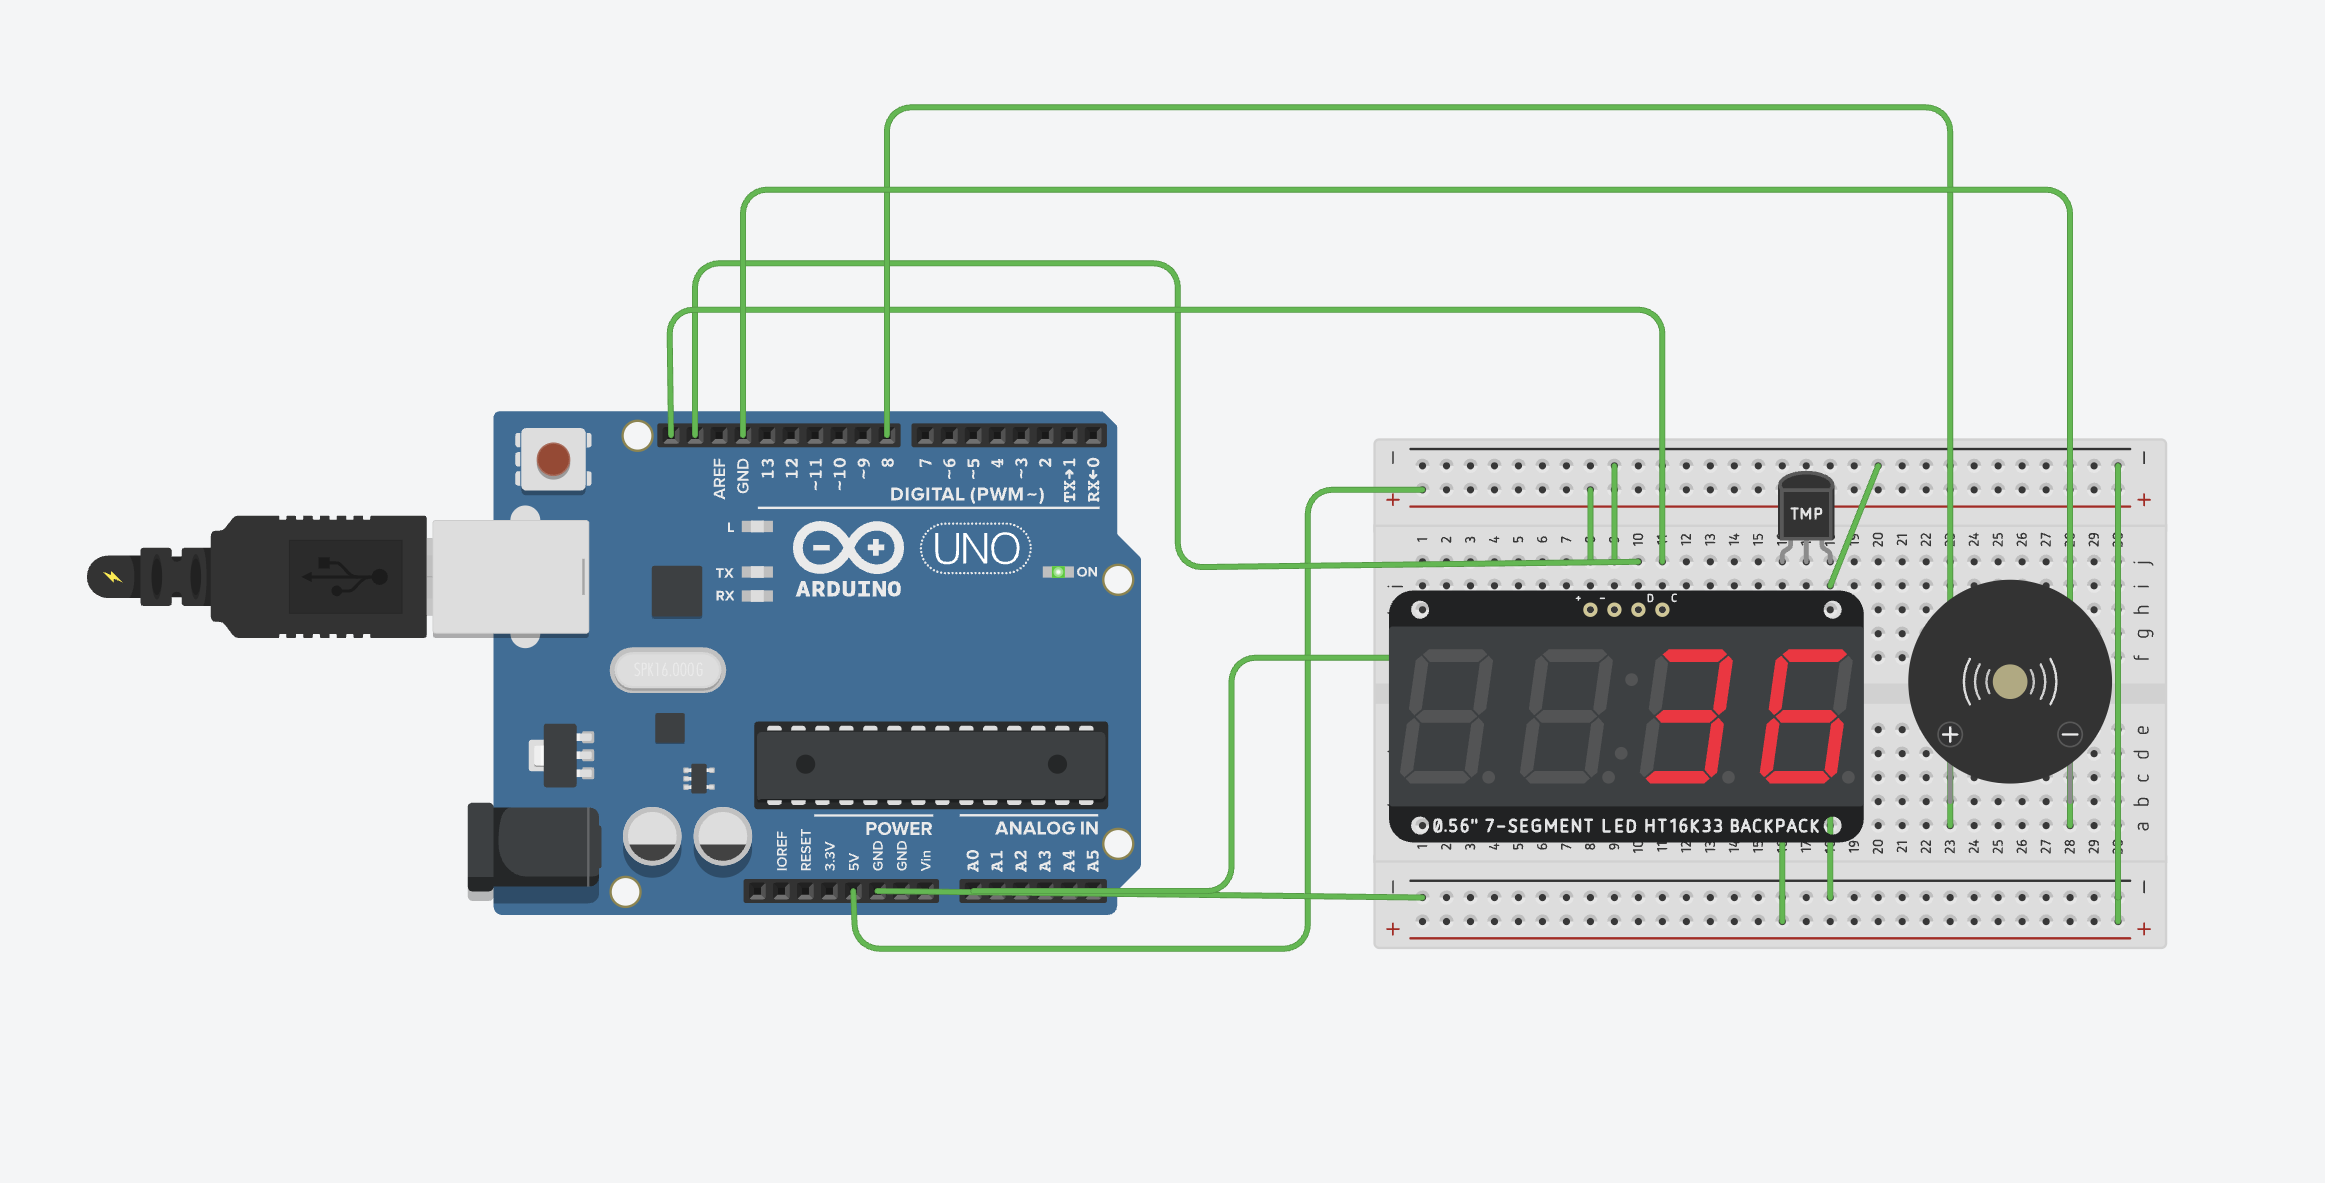
\includegraphics[width=10cm]{./Figs/dousa.png}
\caption{本システムの動作の様子.電圧は5.0Vであり,アナログ値の取得のためにA0ピンに接続されている.
圧電ブザーには8ピンを使用し,7セグメントディスプレイにはSDAピンとSCLピンを使用している.なお,7セグメントディスプレイは0x70のアドレスで接続されている.}
\label{fig:problem}
\end{figure}


\indent
本システムの構成要素を表\ref{table:presentation}に,動作の様子を図\ref{fig:problem}に示す.
まず入力として,温度センサー[TMP36]を用いて,A0ピンから温度センサーのアナログ電圧を取得する.
次に,温度センサーからのアナログ電圧をArduino UNO R3でデジタル値に変換し,気温を算出する.
アナログ電圧から気温を算出する式は(1)(2)式の通りである.
\begin{equation}
V_{\text{in}} = \frac{\text{analogRead}(A0)}{1023} \times V_{\text{ref}}
\end{equation}

\begin{equation}
T\;[^{\circ}C] = (V_{\text{in}} - 0.5) \times 100
\end{equation}

\indent
ここで,$V_{\text{ref}}$はArduino UNO R3の基準電圧5.0Vであり,$T$は気温である.
また,(1)(2)式から求められた気温をもとに,7セグメントディスプレイの表示制御と圧電ブザーのアラーム制御を行う.
これらの一連の処理はArduino UNO R3のプログラムにより実行される.
最後に,7セグメントディスプレイと圧電ブザーで出力を行う.

\subsection{プログラムの概要}

\begin{figure}[H]
\centering
\begin{lstlisting}[firstnumber=1, caption=Arduino UNO R3のソースコード, label=code]
#include <Adafruit_LEDBackpack.h>
#include <Wire.h>

const float vRef = 5.0;

Adafruit_7segment ht = Adafruit_7segment();

void setup() {
  Serial.begin(9600);
  pinMode(A0, INPUT);
  pinMode(8, OUTPUT);

  ht.begin(0x70);  
}

int readtemperatureC(int pin){ 
  
  int ad = analogRead(pin);

  float voltage = ad * vRef / 1023.0;
  int temperatureC = (voltage - 0.5) * 100.0;
  
  return temperatureC;
  } // ピンから取得したアナログ値を基に気温を算出する関数

void loop() {
  int temperatureC=readtemperatureC(A0);

  ht.print((int)temperatureC);  // 気温を整数で表示

  ht.writeDisplay();  //ディスプレイ上に表示
  
  if (temperatureC > 30) {
    
    tone(8, 523);
    delay(600);
    noTone(8);
    delay(600);
  }
}
\end{lstlisting}
\end{figure}

\subsubsection{プログラム全体の説明}
\indent
Arduino UNO R3のプログラムは上記のとおりである.
また,本システムで使用したライブラリはAdafruit\_LEDBackpackとWireであり,
プログラム全体の概要は以下の通りである.
\begin{itemize}
\item 初期化処理として,シリアル通信の開始,A0ピンの入力モード設定,8ピンの出力モード設定,7セグメントディスプレイの初期化を行う.
\item ループ処理では,まずA0ピンからアナログ値を読み取り,それを基に電圧を計算する.
\item 次に,計算した電圧から気温を算出する.
\item 7セグメントディスプレイに気温を表示する.
\item 気温が30度を超えた場合、圧電ブザーを鳴らして警告する.
\item 圧電ブザーは523Hzの音を600ミリ秒間鳴らし、2回繰り返す.
\end{itemize}

\subsubsection{関数の説明}
\begin{table}[H]
  \centering
  \caption{使用した関数の一覧}
  \label{table:functions}
  \begin{tabular}{cccl}
\hline
関数名 & 引数 & 戻り値 & 機能\\\hline \hline
Serial.begin & baudrate & void & シリアル通信を開始する\\ \hline
analogRead & pin & int & 指定したピンのアナログ値を読み取る\\ \hline
pinMode & pin, mode & void & 指定したピンのモードを設定する\\ \hline
ht.begin & address & void & 7セグメントディスプレを初期化する\\ \hline
ht.print & value & void & 7セグメントディスプレイに値を表示する\\ \hline
ht.writeDisplay & なし & void & 7セグメントディスプレイに表示を反映する\\ \hline
tone & pin, frequency & void & 指定したピンで指定した周波数の音を鳴らす\\ \hline
noTone & pin & void & 指定したピンの音を止める\\ \hline
delay & milliseconds & void & 指定した時間だけ処理を停止する\\ \hline
readtemperatureC & pin & int & 指定したピンからアナログ値を読み取り、気温を算出する\\ \hline
\end{tabular}
\end{table}

\indent
本システムで使用した関数の説明を表\ref{table:functions}に示す.
まず,Listing1の8行目から14行目のsetup関数内では,Serial.beginによるシリアル通信の開始,pinModeによるA0ピンの入力モード設定と8ピンの出力モード設定,ht.beginによる7セグメントディスプレイの初期化を行う.
Serial.beginでは引数としてボーレートを指定し,今回は9600bpsを指定している.
pinModeでは引数としてピン番号とモードを指定し,A0ピンは入力モード,8ピンは出力モードに設定している.
ht.beginでは引数として7セグメントディスプレイのアドレスを指定し,今回は0x70を指定している.
次に,16行目から24行目では,電圧のアナログ値を読み取り,気温を算出するreadtemperatureC関数を定義している.
この関数では,analogRead関数を使用してA0ピンからアナログ値を取得し,それを基に電圧を計算している.また,引数はピン番号であり,
その後は計算した電圧から気温を算出し,整数値として返す処理を行っている.
26行目から46行目のloop関数では,気温を7セグメントディスプレイに表示させたり圧電ブザーを鳴らすための制御を行っているが,
27行目では前述したreadtemperatureC関数を呼び出してA0ピンから気温を取得し,temperatureC変数に格納している.
その後,ht.print関数を使用して7セグメントディスプレイに気温を表示し,ht.writeDisplay関数で表示を反映させている.
さらに33行目からは,if文を使用して気温が30度を超えた場合には圧電ブザーを鳴らす処理を行っている.
圧電ブザーはtone関数を使用して8ピンで523Hzの音を600ミリ秒間鳴らし,noTone関数で音を止めた後,さらに600ミリ秒間の待機を行っており,
これらの処理によって圧電ブザーのアラームを実現している.

\section{本システムの実動作}
\begin{figure}[H]
\centering
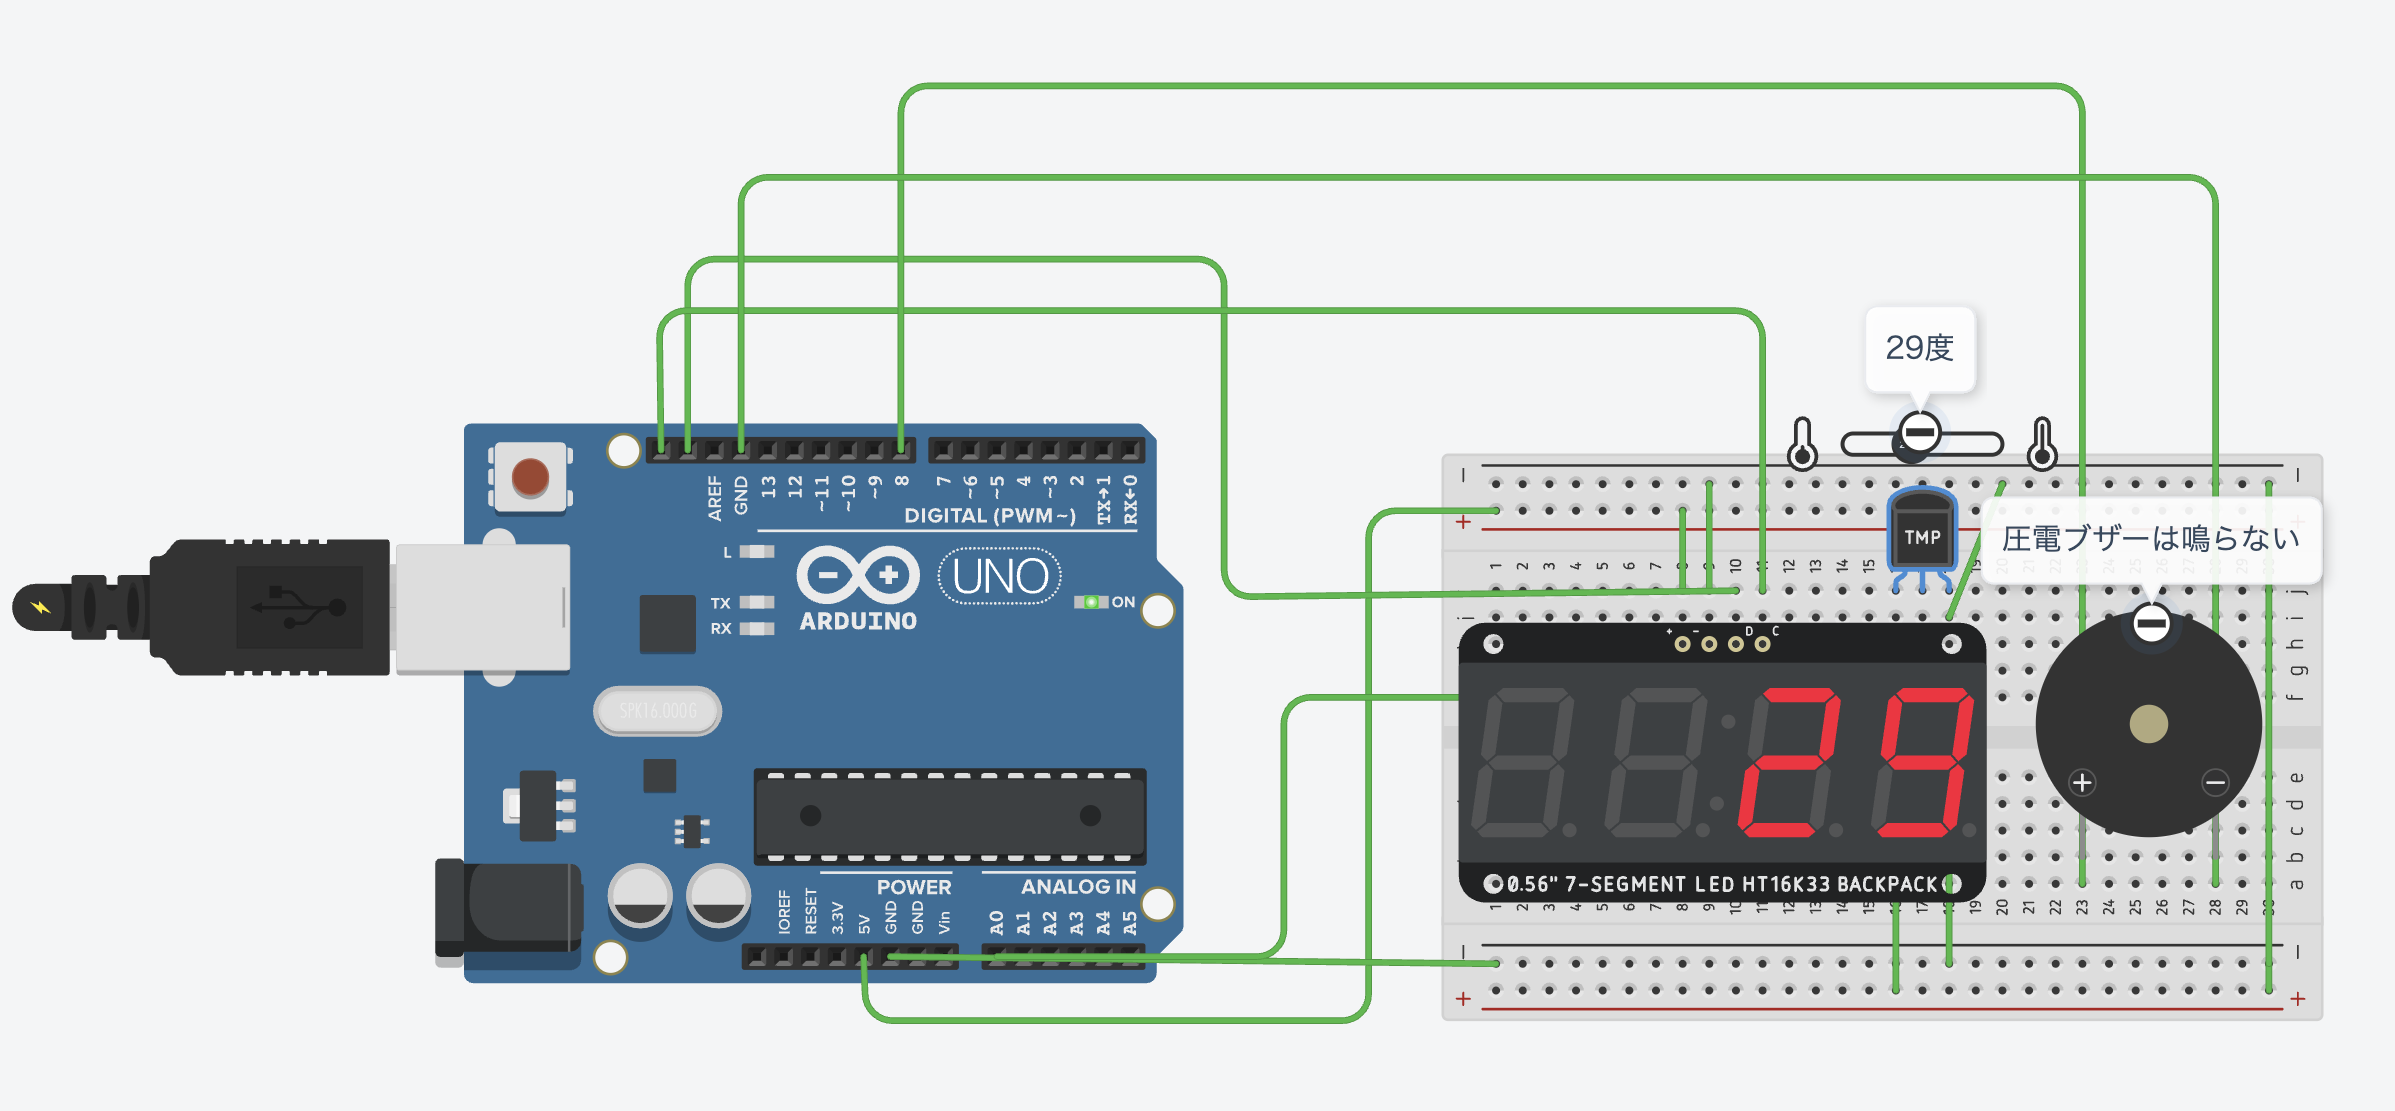
\includegraphics[width=1.0\linewidth]{./Figs/30low.png}
\caption{30度以下の気温でのシステムの動作.}
\label{fig:30low}
\end{figure}
\begin{figure}[H]
\centering
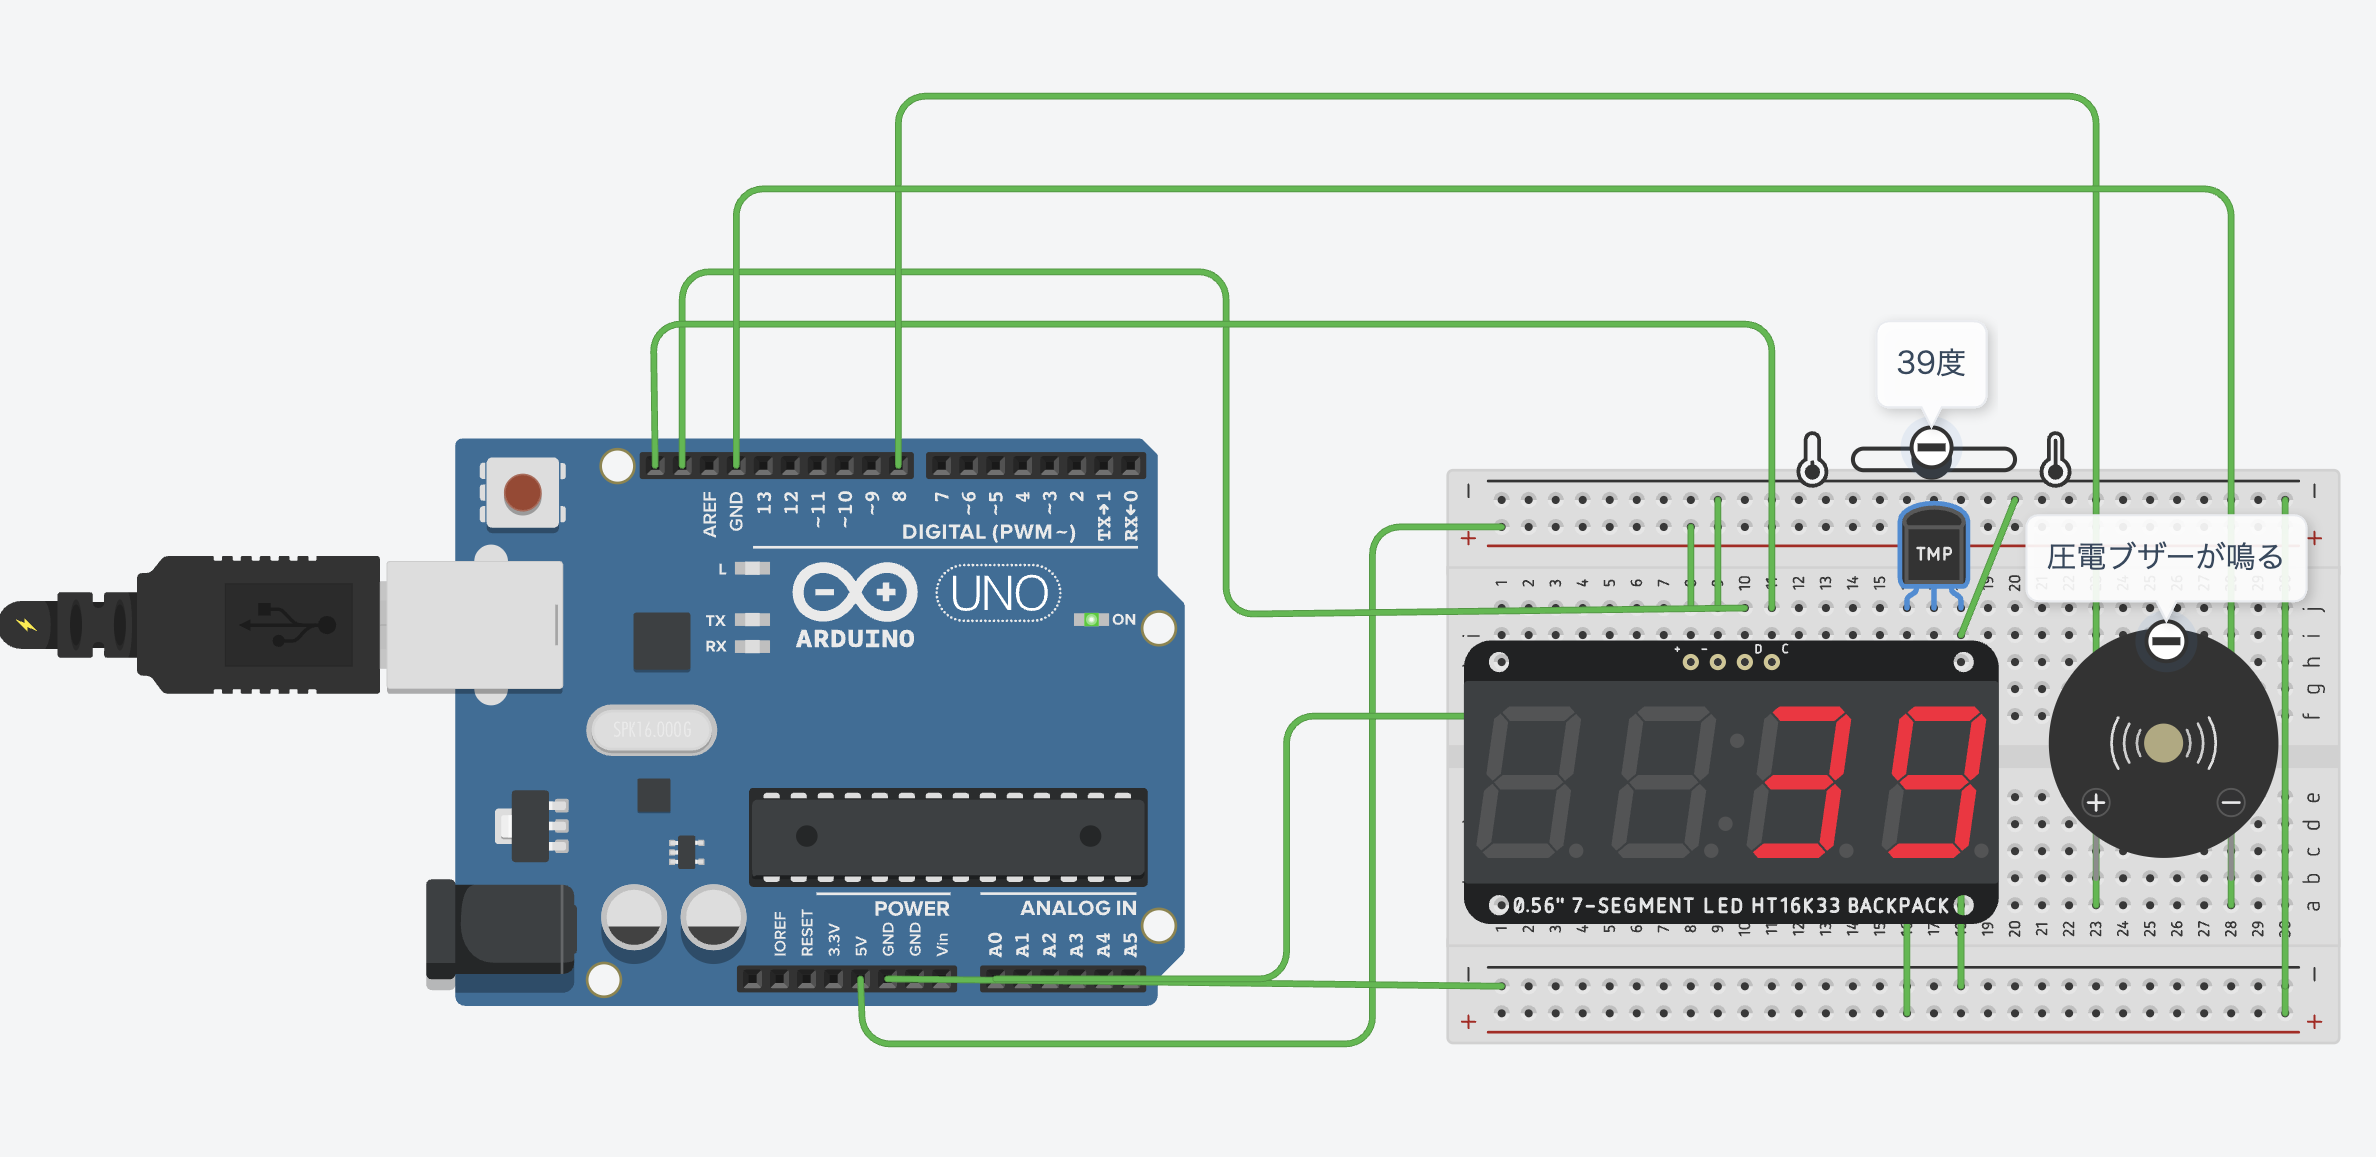
\includegraphics[width=1.0\linewidth]{./Figs/30high.png}
\caption{30度を超える気温でのシステムの動作.}
\label{fig:30high}
\end{figure}

\indent
本システムの実動作を図\ref{fig:30low}と図\ref{fig:30high}に示す.
図\ref{fig:30low}は30度以下の気温でのシステムの動作を示しており,7セグメントディスプレイには30度以下の気温が表示されている.
この場合、圧電ブザーは鳴らず,システムは正常に動作していることが確認できる.
一方、図\ref{fig:30high}は30度を超える気温でのシステムの動作を示しており,7セグメントディスプレイには30度を超える気温が表示されている.
この場合、圧電ブザーが鳴り、アラームで警告が行われていることが確認できる.

\section{本システムのアピールポイント}
\indent
本システムは,講義内で用いた温度センサーと7セグメントディスプレイ・圧電ブザーを組み合わせて,気温のリアルタイム表示とアラームによる警告を実現している点が特徴である.
特に,7セグメントディスプレイは講義内では固定の値を表示するために使用されていたが,本システムでは温度センサーからの入力値を変換し,求められた気温を変数として扱うことで,リアルタイムに表示することが可能となっている.
また,これらの要素の組み合わせは,熱中症対策という当初の目的に対して効果的なものとなっており,システムとしての実現可能性と妥当性もあると考えられる.

\section{注意事項}
\indent
本システムの温度検知において,Arduino UNO R3の処理によって求められた気温は,小数点以下を切り捨てた整数値であるため,表示される温度は実際の温度よりも低くなる場合がある.
そのため,表示される温度が30度を超えた場合でも,実際の温度が30度以下である可能性があることに注意が必要である.
また,圧電ブザーの音量はArduino UNO R3の出力電圧に依存するため、環境によっては音が小さく感じられることがある.
そのため、圧電ブザーの音量を調整するためには、ブザーの電源電圧を変更するか、ブザー自体の仕様を確認する必要がある.
さらに、7セグメントディスプレイの表示は、Arduino UNO R3の処理速度に依存するため、表示が遅れることがあり,表示が遅れる場合はプログラムの処理速度を調整するか、7セグメントディスプレイの仕様を確認する必要がある.

\section{おわりに}
\indent
本稿では,高気温時警告システムの概要や構成,プログラムの説明,実動作の様子を示した.
本システムは,気温のリアルタイム表示とアラームによる警告を実現しており,熱中症対策に有効であると考えられる.
実際の環境での使用にあたっては,注意事項を考慮し,適切な設定や調整を行うことが重要である.
また,今回はアクチュエータとして圧電ブザーを使用したが,より大きな音量が必要な場合はスピーカーなどの他のアクチュエータを使用することも検討できる.
単純なシステムであるが単純故に拡張性が高く,今後の改良や機能追加が容易であり,さらなる発展が期待できる.

\section{TinkerCadのリンク}
\url{https://www.tinkercad.com/things/6XujYAWZ3oc-/editel?returnTo=%2Fdashboard%2Fdesigns%2Fcircuits&sharecode=rltL3EJg_tPyliN_Yu4awmc0KybTstgs-JpTvKHY65Y}
\end{document}
